\date{}
\section{Topologi Jaringan \textit{Cloud Computing}}
Berbicara tentang sistem \textit{Cloud computing}, akan sangat membantu bila kita membaginya menjadi dua kelompok, yakni : front-end dan back-end. Keduanya terhubung melalui sebuah jaringan (Internet). Front-end terletak pada sisi pengguna atau client. Sementara back-end adalah bagian "awan" dalam sistem ini (dalam diagram jaringan internet kerap digambarkan sebagai awan).\\
\tab Front-end mencakup komputer (atau jaringan komputer) client, dan aplikasi yang diperlukan untuk mengakses sistem \textit{Cloud computing}. Tidak semua sistem \textit{Cloud computing} memilikin interface yang sama. Untuk mengakses layanan Web 2.0 seperti email berbasis web hanya dibutuhkan web browser biasa, seperti Firefox, Internet Explorer, atau  Opera.
Namun, adapula sistem\textit{Cloud computing} yang memiliki aplikasi sendiri \textit{(proprietary)} yang harus diinstall di komputer client. Sementara itu, pada sisi backend dari sistem \textit{Cloud computing} terdapat beragam komputer, server, dan sistempenyimpanan data, yang kesemuanya menciptakan "awan" bagi layanan komputasi.
\\
\tab Secara teori, sebuah sistem\textit{Cloud computing} mencakup semua programkomputer yang dapat Anda bayangkan, dari data processing hingga video game. Biasanya, setiap aplikasi dijalankan dan memiliki server sendiri (dedicated server). Sebuah server pusat mengatur jalannya sistem, seperti memonitor lalu lintas, dan permintaan client untuk memastikan semuanya berjalan dengan baik.\\
Bila sebuah perusahaan \textit{Cloud Computing} memiliki banyak client, maka kebutuhan akan ruang penyimpanan data (storage space) pun akan membengkak. Sistem \textit{Cloud Computing} paling tidak membutuhkan ruang penyimpanan data dua kali lebih besar daripada kebutuhan riil untuk membuat salinan (copy) semua data client. Hal ini dimaksudkan untuk mencegah kehilangan data bila terjadi gangguan pada media penyimpanan utama.\\

\begin{center}
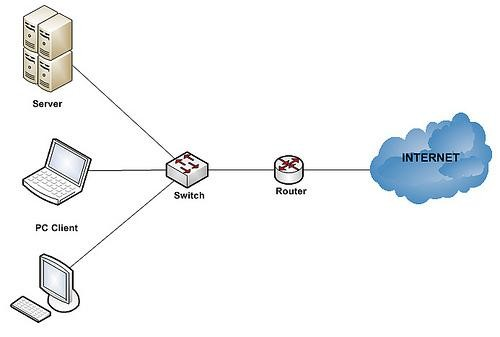
\includegraphics[scale=1]{gambar21.jpg} \\
\textbf{Gambar  2.1} gambaran umum topologi \textit{Cloud computing}
\end{center}
\textbf{Distribusi beban vertikal untuk Komputasi Awan melalui Pilihan Implementasi  Multiple.}
\\\\
\textit{Cloud Computing} menyediakan perangkat lunak sebagai layanan "cadangan" untuk pengguna terakhir, tapi infrastruktur yang mendasari harus cukup terukur dan kuat.dan harus fokus pada sistem \textit{Cloud} perusahaan skala besar dan meneliti  bagaimana  perusahaan dapat menggunakan service-oriented architecture (SOA) untuk menyediakan antarmuka yang efisien untuk proses bisnis.\\
\tab Untuk meningkatkan proses bisnis, masing-masing tingkatan SOA biasanya menyebarkan beberapa server untuk muatan distribusi dan toleransi kesalahan. Salah satu keterbatasan dari pendekatan ini adalah beban yang tidak dapat didistribusikan lebih lanjut saat semua server pada tingkatan /jajaran yang sama dimuat.\\
\textit{Cloud computing} terlihat untuk perhitungan dan penyimpanan data menjauh dari end user dan ke server yang berlokasi di pusat data, dengan demikian mengurangi beban pengguna dari penyedian aplikasi dan manajemen. \\
\tab Dalam sistem awan enterprise, arsitektur berorientasi layanan  (SOA)  dapat digunakan untuk menyediakan antarmuka yang mendasari proses bisnis, yang ditawarkan melalui awan(\textit{cloud}). SOA dapat bertindak sebagai sebuah front-end terprogramke berbagai komponen layanan yang dibedakan           sebagai individu dan pendukung server. Permintaan yang masuk ke layanan yang disediakan oleh gabungan SOA harus diteruskan ke komponen yang benar dan server masing-masing, dan seperti routing harus  terukur untuk mendukung sejumlah besar  permintaan.\\
Dalam rangka untuk meningkatkan proses bisnis, setiap tingkatan dalam sistem biasanya menyebarkan beberapa server untuk mendistribusikan beban dan toleransi kesalahan. seperti distribusi beban di beberapa server dalam tingkat yang sama dapat dilihat sebagai distribusi beban horisontal, tampak seperti gambar berikut :\\
\begin{center}
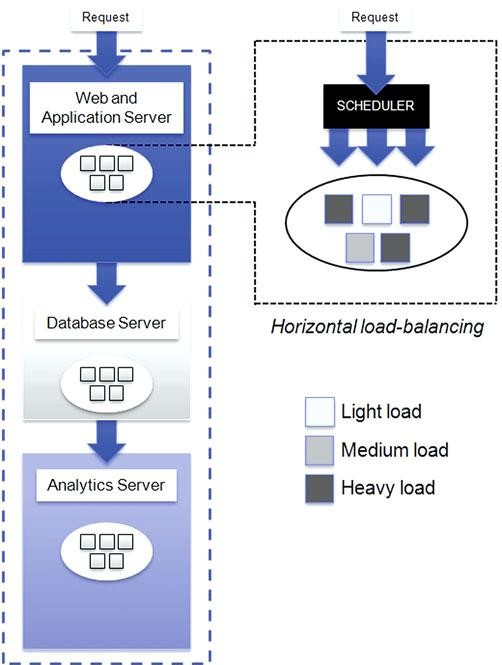
\includegraphics[scale=1]{gambar22.jpg} \\
\textbf{Gambar 2.2} Horizontal distribusi beban: beban didistribusikan di dalamserver, dalamtingkat yang sama.
\end{center}
Salah satu batasan dari distribusi beban horisontal adalah bahwa beban tidak dapat didistribusikan lebih lanjut ketika semua server dalam tingkatan tertentu mengambil hasil dari kesalahan konfigurasi infrastruktur. dimana terlalu banyak server yang dikerahkan pada satu tingkat sementara dilain pihak ada sedikit server yang dikerahkan di lain tingkatan.\\
\tab Sebuah pengamatan penting adalah bahwa dalam sistem kompleks SOA multi-tier, proses bisnis tunggal sebenarnya bisa dilaksanakan oleh beberapa jalur yang berbeda melalui tingkat perhitungan dalamrangka memberikan ketahanan dan skalabilitas.\\
Sebuah layanan komposit dapat direpresentasikan sebagai tingkatan pemanggilan beberapa komponen dalam sebuah infrastruktur TI berbasis SOA. Dalam sistem seperti itu, kami membedakan distribusi beban horisontal, dimana beban dapat tersebar di  beberapa  server untuk satu komponen layanan, dari distribusi beban vertical, dimana beban dapat tersebar di beberapa implementasi dari layanan yang diberikan. Gambar berikut menggambarkan istilah- istilah di atas.\\\\
\begin{center}
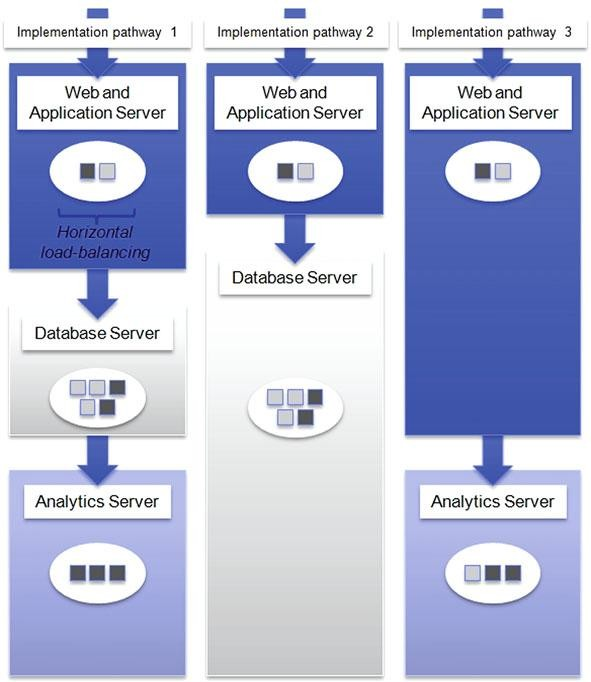
\includegraphics[scale=1]{gambar23.jpg} \\
\textbf{Gambar  2.3} Distribusi beban vertical.
\end{center}
Berikut tugas analitik komposit online dapat direpresentasikan sebagai panggilan  untuk Web  dan Aplikasi Server (WAS) untuk melakukan pra-pemrosesan tertentu, diikuti dengan sebuah panggilan dari WAS ke server database (DB) untuk mengambil  data yang dibutuhkan,  setelah itu WAS meneruskan data yang ditetapkan ke server analitik khusus untuk tugas-tugas komputasi data mining yang mahal.\\
\tab Tugas komposit memiliki beberapa implementasi di pusat data modern IT. Implementasi alternatif dapat memanggil prosedur yang tersimpan pada database untuk menjalankan data mining dan bukan memiliki server analitik khusus untuk melakukan tugas ini. Implementasi alternatif menyediakan distribusi     beban vertikal dengan memungkinkan penjadwalan pekerjaan untuk memilih\ implementasi WAS-dan-DB saat analitik server tidak tersedia.\\
\textit{Reusability} adalah salah satu tujuan utama dari pendekatan SOA. Sehubungan dengan reusability yang tinggi dari komponen aplikasi, adalah mungkin untuk menentukan alur kerja yang kompleks dengan beberapa cara. Namun sulit untuk menilai, mana yang merupakan penerapan yang terbaik.\\
Pada bagian ini diberikan gambaran sistem arsitektur dan contoh komputasi awan yang disederhanakan(seperti  gambar berikut).\\
\begin{center}
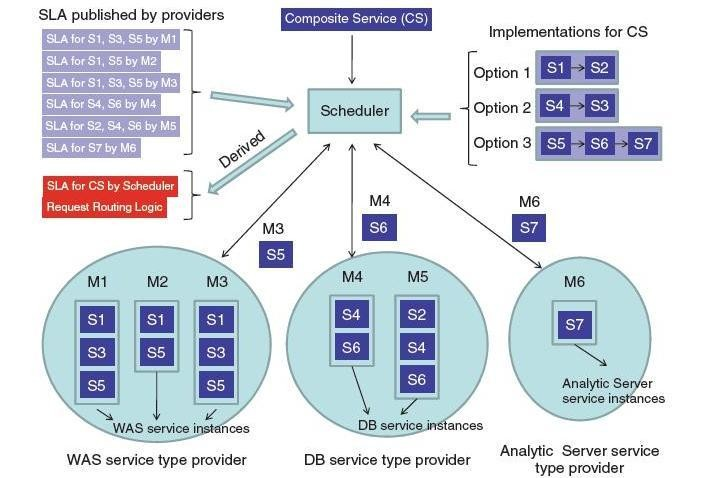
\includegraphics[scale=1]{gambar24.jpg} \\
\textbf{Gambar  2.4} Request routing for SOA-based enterprise computing with multiple implementation options.
\end{center}
di mana sebuah proses analitik berjalan pada Web dan Aplikasi Server (WAS),  Database  Server (DB), dan Server Analytic khusus. proses analitik dapat diimplementasikan  oleh salah satu dari tiga pilihan (seperti yang ditunjukkan pada gambar di atas):
\begin{itemize}
\item Mengeksekusi beberapa pra-pengolahan di WAS (S1) dan kemudian memiliki DB untuk menyelesaikan perhitungan analitik (S2); atau
\item Mengambil data dari DB (S4) ke WAS dan kemudian menyelesaikan sebagian besar perhitungan analitik di WAS (S3); atau
\item Mengeksekusi  beberapa   pra-pengolahan   di  WAS   (S5),   dan   kemudian   memiliki DB setelah itu mengambil data yang diperlukan (S6), dan akhirnya menampilkan AS untuk   melakukan perhitungan sisa analitik(S7).
\end{itemize}
Proses analitik memerlukan tiga jenis layanan yang berbeda, yaitu layanan jenis WAS, layanan jenis DB, dan layanan jenis AS. S1, S3, dan S5 adalah contoh dari jenis layanan WAS karena mereka adalah layanan yang diberikan/disediakan oleh WAS \textit{(Web and Application Server)}. Demikian pula, S2, S4, dan S6 merupakan contoh dari jenis layanan DB\textit{(Database Server)}, dan S7 adalah turunan dari jenis layanan AS \textit{(Analytic Server)}.\\
\tab Selain itu, ada tiga jenis server: WS server (M1, M2, dan M3); DB server (M4 dan M5), dan AS server (M6). Meskipun server dapat mendukung hal lain dari jenis layanan yang diberikan, secara umum hal ini tidak selalu terjadi. Sebagai contoh : setiap server dapat mendukung semua contoh jenis layanan perusahaan, kecuali M2 dan M4 adalah server yang kurang kuat sehingga mereka tidak dapat mendukung layanan komputasi yang mahal , S3 dan S2.\\
\tab Setiap server memiliki \textit{Service Level Agreement} (SLA) untuk setiap contoh layanan yang mendukung, dan SLA ini diterbitkan dan tersedia untuk penjadwal. SLA termasuk informasi seperti beban profil versus waktu respon dan batas atas permintaan ukuran beban  dimana server dapat memberikan jaminan waktu respon nya.\\
\textit{Scheduler} bertanggung jawab untuk routing dan mengkoordinasikan pelaksanaan pelayanan komposit/gabungan dari satu atau lebih implementasi. Sebuah SLA yang diperoleh hanya dapat digunakan sesuai logika routing. \textit{Scheduler} dapat memperoleh SLA dan logika routing serta menangani permintaan routing. Atau, \textit{Scheduler} dapat digunakan hanya untuk tujuan menurunkan SLA dan logika routing saat mengkonfigurasi isi router , seperti  (Cisco System  Inc), untuk kinerja tinggi dan hardware berbasis routing.\\
\tab \textit{Scheduler} juga dapat ditingkatkan untuk melakukan tugas pemantauan yang actual dari QoS \textit{(Quality of Service)} yang dicapai oleh eksekusi alur kerja dan oleh penyedia layanan individu. Jika \textit{scheduler} mengamati kegagalan penyedia layanan tertentu untuk QoS yang dipublikasikan, dapat menghitung kembali kelayakan dari QoS dan logika routing sesuai kebutuhan/permintaan yang dapat   beradaptasi dengan lingkungan  runtime.
\section{Perangkat Lunak \textit{Cloud Computing}}
\textbf{\textit{OpenStack,} perangkat lunak \textit{Cloud computing} Open  Source.}\\\\
\textit{OpenStack} merupakan open source \textit{\textit{\textit{Cloud}computing}} software untuk membangun infrastruktur \textit{Cloud}yang reliabel dimana baru saja dipublikasikan beberapa hari lalu yaitu pada tanggal 19 Juli 2010. Tujuan OpenStack adalah untuk memungkinkan setiap organisasi atau perusahaan untuk membuat dan menyediakan layanan \textit{Cloud computing} dengan menggunakan perangkat lunak open source yang berjalan diatas perankat keras yang standar.\\
\tab Terdapat dua jenis OpenStack, yaitu OpenStack Compute dan OpenStack Storage. OpenStack Compute adalah perangkat lunak untuk melakukan otomasi saat membuat ataupun mengelola virtual private server (VPS) dalam jumlah besar. Sedangkan OpenStack Storage adalah perangkat lunak untuk membuat object storage yang bersifat scalable serta redundant dengan menggunakan cluster untuk menyimpan data data dalamukuran terabytes atau bahkan petabytes.\\
Seluruh kode OpenStack berada dibawah lisensi Apache 2.0. Sehingga  memungkinkan siapapun untuk menjalankan, membangun perangkat lunak lain diatas perangkat lunak OpenStack atau mengirimkan perubahaan kode entah sebagai  patch atau fitur baru.\\
\tab OpenStack saat ini telah digunakan perusahaan besar hosting seperti  Rackspace Hosting dan NASA. Mereka menggunakan teknologi OpenStack untuk mengelola puluhan ribu compute instance dan storage dalamukuran petabytes.\\\\
\textbf{\textit{Amazon Elastic Compute \textit{Cloud}(EC2).}}\\\\
Amazon telah memberikan solusi universal dan komprehensif yang populer untuk \textit{Cloud computing}, yang disebut Amazon Elastic Compute \textit{Cloud}(EC2) (2010). Solusi ini dirilis sebagai versi "beta" umumyang terbatas pada tanggal 25 Agustus 2006, tetapi tumbuh pesat di tahun- tahun berikutnya.\\
\tab EC2 menyediakan banyak fitur yang berguna bagi pelanggan, termasuk sistem penagihan yang terencana dan biaya untuk komputasi yang murah pada tingkat yang sangat mantap (penggunaan memori, penggunaan CPU, transfer data, dll), penyebaran antara beberapa lokasi, elastis alamat IP, infrastruktur yang ada sambungan ke pelanggan melalui Virtual Private Network (VPN), jasa pemantauan oleh \textit{Amazon CloudWatch}, dan \textit{load balancing} elastis. Amazon‘s EC2 provides virtual machine based computation environments. EC2 menggunakan hypervisor Xen (2010) untuk mengelola Amazon Mesin Gambar (AMI). AMI (Amazon EC2, 2010) adalah "gambar terenkripsi mesin yang berisi semua informasi yang diperlukan untuk perangkat lunak yang kita pakai ". Dengan menggunakan interface layanan web sederhana, pengguna dapat memulai, menjalankan, memonitor dan menghentikan kasus mereka seperti ditunjukkan pada Gambar di bawah ini.\\
\begin{center}
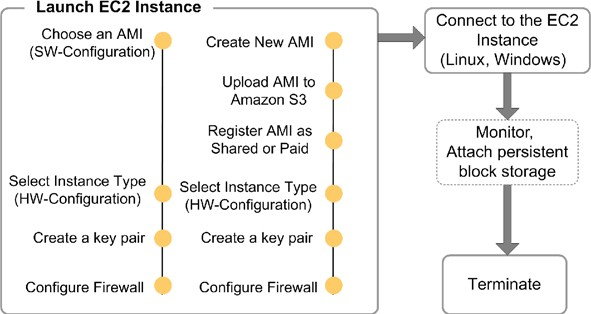
\includegraphics[scale=1]{gambar25.jpg} \\
\textbf{Gambar  2.5} Launch EC2 Instance 
\end{center}
Selain itu mereka dapat dengan cepat menambahkan satu fitur seperti yang disebutkan di atas untuk konfigurasi sesuai  dengan apa yang pengguna inginkan.\\\\
\textbf{GoGrid.}\\\\
GoGrid memiliki  karakteristik umumdengan Amazon di area klasik komputasi  awan,  dalam hal ini mendukung beberapa sistemoperasi melalui gambaran manajemen sendiri, dan mendukung dalamhal menyeimbangkan beban, penyimpanan awan, dan sebagainya. Selain itu, GoGrid menyediakan pelanggan dengan antarmuka web yang user-friendly service, mudah dimengerti demonstrasi video, dan sistempenagihan yang ketat tapi tidak  mahal.\\
Jadi baik EC2 dan GoGrid, kedua-nya menyediakan fitur dasar dan umum dari \textit{Cloud} Computing. Perbedaan antara layanan yang mereka(EC2 dan  GoGrid)  berikan  terutama berasal dari model bisnis mereka masing-masing.\\
Sebagai contoh, GoGrid menyediakan awan(\textit{Cloud}) bebas dan penyimpanan yang spesifik, sedikit berbeda dari Amazon.\\
\tab GoGrid juga menyediakan Hybrid Hosting, yang merupakan fitur pembeda. Banyak aplikasi namun tidak dapat berjalan dengan baik di lingkungan server yang murni  multi-tenant.\\
Performa Database lebih baik pada dedicated server, dimana EC2 dan GoGrid tidak perlu bersaing untuk input / output sumber daya, situasi ini mirip dengan aplikasi web server. GoGrid menyediakan aplikasi-aplikasi khusus dengan dedicated server  yang memiliki  jaminan keamanan yang tinggi.\\\\
\textbf{\textit{Amazon Simple Storage Service (S3).}}\\\\
Amazon Simple Storage Service (2010) (S3) adalah layanan web penyimpanan online yang ditawarkan oleh Amazon Web Services. S3 dapat diakses pengguna melalui layanan web, REST-style interface HTTP, atau dengan melibatkan antarmuka SOAP. Seperti halnya layanan komputasi awan lainnya, pengguna dapat meminta penyimpanan dalamjumlah kecil atau besar dengan cepat, serta menyediakan sistempenyimpanan sangat  terukur.\\
\tab Amazon S3 mengatur ruang penyimpanan ke dalam banyak kotak, dengan setiap kotak diberi namespace yang pada umunya unik dengan maksud untuk membantu menemukan  alamat data, mengidentifikasi \textit{user account} untuk pembayaran, dan mengumpulkan informasi penggunaan. Amazon S3 berurusan dengan semua jenis data sebagai obyek. Sebuah objek dapat diakses melalui URL yang terdiri dari kunci dan versi ID dengan \textit{namespace} sebagai awalan.\\
Pengguna Amazon S3 tersebar di banyak bidang, misalnya, SmugMug, Slideshare dan Twitter. Twitter menggunakan Amazon S3 untuk \textit{host images}, Apache Hadoop menggunakan S3 untuk menyimpan data komputasi, dan utilitas sinkronisasi online seperti Dropbox dan Ubuntu One gunakan Amazon S3 sebagai  tempat penyimpanan dan fasilitas transfer.\\\\
\textbf{\textit{Rackspace Cloud.}}\\\\
Rackspace Awan awalnya diluncurkan pada tanggal 4 Maret 2006 dengan nama "Mosso". Dalam tiga tahun berikutnya, ia(\textit{Raskspace Cloud}) telah mengubah namanya dari "Mosso LLC" menjadi "Mosso: \textit{The Hosting Cloud}", dan akhirnya menjadi "\textit{Rackspace Cloud}" pada  tanggal  17 Juni 2009.\\
\tab Perusahaan  ini  menyediakan layanan  termasuk   \textit{Cloud server},   \textit{Cloud  file},   dan  \textit{Clousite}. \textit{Cloudfile service} adalah layanan penyimpanan awan\textit{(cloud)} yang menyediakan penyimpanan  online yang tak  terbatas  dan  Jaringan Pengiriman  Konten  untuk media  secara komputasi utilitas. Selain control panel online, perusahaan ini menyediakan layanan API\textit{(Application Programming Interface)} yang dapat diakses melalui \textit{Application Programming Interface} yang aman dengan kode klien \textit{open source}.\\
Rackspace memecahkan masalah keamanan dengan mereplikasi tiga salinan penuh data di beberapa komputer pada beberapa zona, dengan setiap tindakan yang dilindungi oleh SSL\textit{(Secure Socket Layer)}.\\\\
\textbf{\textit{Google App Engine.}}\\\\
\textit{Google App Engine} (GAE) tujuan utama adalah untuk mengefisienkan pengguna menjalankan aplikasi web. Seperti yang ditunjukkan pada gambar berikut.\\
\begin{center}
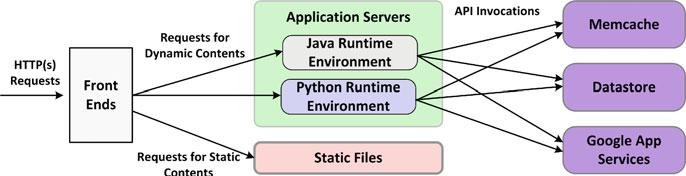
\includegraphics[scale=1]{gambar26.jpg} \\
\textbf{Gambar  2.6} Arsitektur dari \textit{Google App Engine}
\end{center}
\textit{Google App Engine} mempertahankan \textit{Python} dan lingkungan runtime Java  pada  server aplikasi, bersama dengan beberapa \textit{Application Programming Interface} sederhana untuk mengakses layanan Google.\\
\tab Selanjutnya menyebar permintaan HTTP dengan load balancing dan  routing  strategi yang didasarkan pada \textit{Contents}(isi). Runtime sistem yang berjalan pada aplikasi server yang ideal dengan pengolahan logika aplikasi dan menyediakan konten web dinamis, sedangkan halaman statis dilayani  bersama oleh infrastruktur Google.\\
Untuk memisahkan data terus-menerus dari server aplikasi, GAE ( \textit{Google App Engine} ) menempatkan data ke dalam Datastore dari sistem file lokal. Aplikasi dapat mengintegrasikan layanan data dan \textit{Google App} Layanan lainnya, seperti email, penyimpanan  foto  dan sebagainya melalui API ( \textit{Application Programming Interface} ) yang disediakan oleh GAE ( \textit{Google App Engine} ).\\
Selain layanan, Google juga menyediakan beberapa tool untuk pengembang dalam hal ini membantu mereka (pengembang) membangun aplikasi web dengan mudah di GAE (\textit{ Google App Engine} ). Namun, sejak mereka (pengembang) erat terhubung ke infrastruktur Google, ada beberapa pembatasan yang membatasi fungsionalitas dan portabilitas dari  aplikasi.\\
\textbf{Microsoft Azure.}\\\\
Strategi awan Microsoft adalah untuk membangun sebuah  platform  awan  yang mana pengguna dapat memindahkan aplikasi mereka ke dalam cara yang sempurna, dan memastikan bahwa sumber daya yang dikelola dapat diakses untuk kedua layanan awan tersebut   pada aplikasi lokal.\\
\tab Untuk mencapai ini, Microsoft memperkenalkan Windows Azure Platform (WAP), yang terdiri dari sistem operasi Awan(\textit{Cloud}) yang bernama Windows Azure, dan satu set layanan pendukung, seperti ditunjukan pada gambar  berikut.\\
\begin{center}
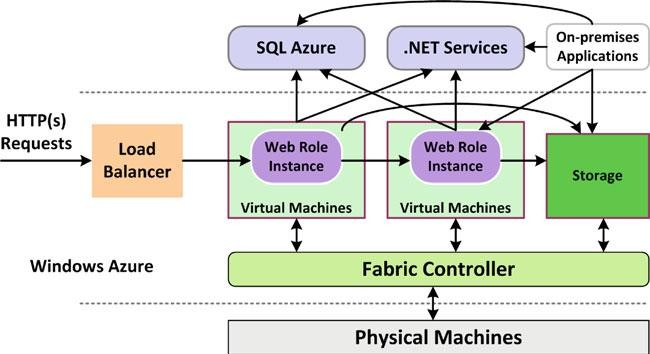
\includegraphics[scale=1]{gambar27.jpg} \\
\textbf{Gambar  2.7} Arsitektur  dari platform Windows Azure
\end{center}
Windows Azure adalah bagian utama dari WAP(\textit{Wireless Application Protocol}). WAP adalah sebuah protokol atau sebuah teknik \textit{messaging service} yang memungkinkan sebuah telepon genggam digital atau \textit{terminal mobile} yang mempunyai fasilitas WAP, melihat/membaca isi sebuah situs di internet dalam sebuah format teks khusus.\\
Ini mempekerjakan mesin virtual sebagai lingkungan runtime nya. Penawaran Aplikasi dalam awan Microsoft dibagi menjadi dua jenis: instansi peran Web, yang dapat melayani permintaan web melalui layanan informasi internet; dan instansi peran pekerja, yang hanya dapat menerima pesan dari instansi peran Web lain atau aplikasi lokal. Windows Azure  mempekerjakan "controller kain" untuk mengelola semua mesin virtual dan server penyimpanan pada mesin fisik di pusat data Microsoft.\\
\tab Windows Azure menggunakan sebuah pengendali kontrol untuk  mengelola  semua mesin virtual dan server penyimpanan pada mesin fisik di pusat data Microsoft. Serupa dengan Datastore di GAE(\textit{Google Application Engine}),WAP(\textit{Wireless Application Protocol}) juga menyediakan layanan database yang disebut SQL Azure, untuk menyimpan data di  awan(\textit{cloud}). Salah satu fitur dari SQL Azure adalah menyediakan alat untuk sinkronisasi data dilokasi lokal.\\
Layanan infrastruktur didukung oleh WAP melalui layanan .NET yang saat ini include dengan kontrol akses dan layanan ekspos. Keduanya tersedia untuk layanan \textit{Cloud}dan layanan lokal.\\
Berikut ini ada 11 top open-source \textit{Cloud}application yang diambil dari GigaOm untuk keperluan pelayanan, pendidikan, support, general itemof interest, dan  lainya.\\
\begin{enumerate}
\item Eucalyptus. Ostatic menggemparkan berita dimana UC Santa Barbara membuat sebuah open-source \textit{Cloud}project tahun kemarin. Dikeluarkan sebagai open-source (dengan menggunakan lisensi FreeBSD-style) Eucalyptus dapat digunakan untuk infrastruktur \textit{Cloud computing} dalam cluster yang dapat menduplikasi fungsionalitas Amazon EC2, Eucalyptus secara langsung menggunakan command-line tool dari Amazon. Sebagai langkah awal Eucalyptus System terlebih dahulu membuat venture funding, untuk  membiayai  staff termasuk arsitek dari Eucalyptus project. Baru baru ini mereka mengeluarkan update software framework nya, yang juga dilengkapi dengan fitur \textit{Cloud computing} yang akan digunakan pada Linux Ubuntu versi terbaru.
\item \textit{Red Hat's Cloud}. Salah satu pemain open-source terlama Red Hat memang telah memfokuskan diri pada \textit{Cloud computing}. Pada akhir juli kemarin,  Red  Hat  membuka sebuah Open Source \textit{Cloud computing} Forum, yang berisi banyak persentasi mengenai ide perpindahan dari open-source untuk mengikuti teknologi cloud.  Anda  dapat  mengikuti  semua free webcast dari semua persentasi Redhat. Pembicaranya Rich Wolski (CTO dari Eucalyptus Systems), Brian Stevens (CTO dari Red Hat), dan juga Mike Olson (CEO dari Cloudera). Steven akan membawa anda mengenai strategi Red Hat terhadap \textit{Cloud computing}. Novell juga open source sedang mencoba untuk memfokuskan ke \textit{Cloud computing}, anda juga dapat  membaca strategi mereka disini.
\item Traffic Server. Yahoo kali ini berpindah ke open-source untuk memberikan inisiatif untuk mewujudkan \textit{Cloud computing} dengan memberikan donasi ke produk \textit{Traffic Server} kepada \textit{Apache Software Foundation}. \textit{Traffic Server} adalah sebuah sistem yang digunakan secara in-house oleh Yahoo untuk mengatur traffic mereka sendiri, dengan ini mereka dapat mengatur \textit{session management, authentication, configuration management, load balancing}, dan juga routing untuk semua \textit{Cloud computing software stack}. Dengan kata lain \textit{Traffic Server} memberikan kemudahan bagi para \textit{IT} administrator untuk mengalokasikan sumber daya, termasuk didalamnya menghandle ratusan dari \textit{virtualized services} secara online.
\item Cloudera. Sebuah \textit{open-source Hadoop software framework} yang saat ini mulai banyak di gunakan pada \textit{Cloud computing deployment} karena fleksibilitas nya yang tinggi dan menggunakan \textit{cluster-based, data-intensive queries tools }ini jadi banyak disukai. Tentu saja ini terlewat oleh I, dan Yahoo juga memiliki \textit{time-tested Hadoop distribution} sendiri. Cloudera nampaknya saat ini menjajikan untuk tahap awal yang memberikan support komersil  untuk Hadoop. anda dapat  membaca tentan Cloudera disini.
\item Puppet. Adalah sebuah teknolosi Virtual server yang dapat di implemetasikan pada \textit{Cloud computing}, dan juga dapat digunakan sebagai \textit{Reductive Lab open-source software} (kurang faham maksudnya apa), software ini dibangun dengan menggunakan \textit{Cfengine system}, dan hebatnya banyak system administrator yang memanfaatkan software ini . Anda dapat dengan mudah mengatur berapapun jumlah virtual machine dan dapat melakukan  automated routine, tampa harus melakukan \textit{complex scripting}.
\item Enomaly. Adalah \textit{Elastic Computing Platform} (ECP) yang merupakan akar dari \textit{ Enomalism open-source provisioning and management software}, teknologi ini di desain untuk mengatur kompleksitas dari implementasi infrastruktur cloud.  ECP  adalah  sebuah  programmable virtual \textit{Cloud computing} infrastructure untuk ukuran kecil, sedang dan juga enterprise besar dan anda dapat  membaca lebih detail disini.
\item 7.	Joyent. Adalah sebuah software yang didirikan pada Januari awal tahun ini, yang memulai open-source  \textit{Cloud} dengan  memanfaatkan  JavaScript  dan  Git.  Infrastruktur  Joyent  cloudhosting dan \textit{Cloudmanagement software} membuka banyak open-source tools untuk public dan private cloud. Perusahaan ini juga membantu mengoptimasi kecepatan  implementasi dari open-source MySQL database untuk penggunaan \textit{Cloud use}.
\item Zoho. Banyak orang mengenal Zoho sebagai free, \textit{online application}, yang menjadi pesaing dari Google Docs. Yang terpenting untuk diketahui adalah bawasanya Zoho core adalah betul betul open source mdash; sebuah contoh bagaimaa solusi SaaS dapat  bekerja  secara harmonis dengan open source. Anda dapat menemukan bagaimana Zoho mengimplementasikan open-source tool melalui interview  mereka.
\item Globus Nimbus. Open-source toolkit ini mampu merubah bisnis anda dari infrastruktur  cluster menjadi Infrastructure-as-a-Service (IaaS) cloud. Amazon EC2 interface digunakan sepenuhnya namun ini bukan hanya sebuah interface yang dapat anda manfaatkan.
\item Reservoir. Adalah sebuah inisiatif dari European research  untuk  mengembangkan virtualized infrastructure and \textit{Cloud computing}. Akhirnya membawa mereka untuk mengembangkan teknologi open-source untuk \textit{Cloud computing}, dan membantu para pengguna bisnis untuk menghemat  biaya IT.
\item OpenNebula. OpenNebula VM Manager adalah sebuah komponen dasasr dari Reservoir. Ia adalah sebuah jawaban open-source untuk berbagai macam jenis virtual machine management yang banyak di gunakan secara proprietary, Interface nya pun dapat dengan mudah dipahami dengan \textit{Cloud infrastructure tools and services}.  "OpenNebula  adalah sebuah open-source virtual infrastructure engine yang akan memberikan anda implementasi dan re-placement dari virtual machines pada physical resources," menurut project lead mereka.
\end{enumerate}
Nampaknya banyak \textit{open-source tools} sudah mulai berkompetisi dalam dunia \textit{Cloud computing}. Hasil akhir dari ini tentu saja nantinya kita akan menemukan fleksibilitas dari organisasi untuk mengkostumasi pendekatan yang mereka inginkan. Open-source \textit{Cloud}akan  memberikan potensi akan harga yang sangat kompetitif  untuk mendapatkan service cloud.
\section{Manajemen  Pengelolaan \textit{Cloud computing}}
Secara teori, sumber daya awan-berbasis layanan tidak harus berbeda dari sumber daya di lingkungan dimana kita berada. Idealnya, Anda memiliki pandangan yang lengkap dari sumber daya yang Anda gunakan saat ini atau mungkin ingin menggunakan di masa depan, namun untuk mencapai ini bukan merupakan sesuatu yang mudah. Dalam lingkungan awan(\textit{cloud}) kebanyakan, pelanggan hanya dapat mengakses layanan, yang berhak mereka  gunakan.\\
Tiga aspek manajemen sumber daya awan(\textit{Cloud Computing}):\\
\begin{itemize}
\item Keamanan TI
\item Kinerja manajemen
\item Provisioning
\end{itemize}
\textbf{Kinerja Manajemen.}\\\\
Manajemen kinerja adalah tentang bagaimana layanan perangkat lunak berjalan efektif  di  dalam lingkungan sendiri(PC sendiri) ataupun melalui awan(\textit{Cloud}). Jika Anda mulai dapat terhubung dengan perangkat lunak yang berjalan di pusat data, lalu Anda sendiri langsung ke perangkat lunak yang berjalan di awan(\textit{Cloud}), kemungkinan besar Anda akan ada potensi kemacetan pada titik koneksi.\\\\
\textbf{Jasa manajemen}\\\\
Jasa manajemen dalamkonteks ini mencakup semua kegiatan operasi data \textit{centre}.\\
Disiplin yang luas ini mempertimbangkan teknik yang diperlukan dalam manajemen \textit{Cloud Computing} dan alat untuk mengelola jasa/layanan oleh penyedia awan(\textit{Cloud}) dan data internal manajer pusat di lingkungan ini, hal –hal yang diperlukan antara lain:\\
\begin{itemize}
\item Fisik
\item TI
\item Virtual
\end{itemize}
Layanan manajemen mencakup berbagai  disiplin,  yaitu :\\
\begin{itemize}
\item Konfigurasi  manajemen
\item Aset Manajemen
\item Jaringan manajemen
\item Kapasitas  perencanaan
\item Analisis akar penyebab
\item Beban Kerja manajemen
\item Patch dan memperbarui manajemen
\end{itemize}
Namun Kenyataannya adalah bahwa \textit{Cloud}itu sendiri adalah sebuah platform manajemen layanan. Oleh karena itu, portofolio layanan \textit{Cloud}dirancang dengan baik  termasuk integrasi ketat dari  kemampuan layanan manajemen inti dan antarmuka yang terdefinisi dengan baik.\\\\
\textbf{Mengelola beban kerja di Awan ( \textit{Cloud})}\\\\
Bagaimana Anda mengatur Teknologi ini (\textit{cloud})? Persyaratan dasar adalah bahwa beban kerja perlu untuk diorganisir.Beban kerja adalah sebuah layanan independen atau kumpulan kode yang dapat dieksekusi.\\
Oleh karena itu, beban kerja tidak perlu bergantung pada unsur luar. Beban kerja bisa menjadi sebuah aplikasi kecil atau lengkap. Dimana kita harus dapat menyeimbangkan dua hal:\\
\begin{itemize}
\item Aplikasi atau komponen yang berjalan di awan(\textit{cloud})
\item Kebutuhan bisnis untuk melakukan perkiraan /estimasi kebutuhan bisnis, terutama saat beban puncak.
\end{itemize} 
Organisasi harus secara aktif mengelola beban kerja sehingga mereka tahu\\
\begin{itemize}
\item Bagaimana aplikasi  mereka berjalan
\item Apa yang mereka lakukan
\item Berapa banyak departemen individu atau UKM harus dikenakan biaya untuk setiap penggunaan layanan \textit{Cloud computing}
\end{itemize}
\tab Setiap provider layanan \textit{Cloud computing} dalam menjalankan jasa bisnis-nya membutuhkan suatu perencanaan untuk beban kerja mereka, bahkan  ketika  perusahaan layanan tersebut sedang menggunakan operator eksternal Cloud. Manajemen perlu memahami jenis beban kerja mereka untuk ditempatkan di \textit{Cloud}.\\
Beban kerja bisa menjadi segalanya dari data intensive untuk penyimpanan beban kerja atau proses transaksi  beban kerja.\\
\tab Hal yang perlu diperhatikan dalammanajemen pengolahan \textit{Cloud computing} adalah
"Mendeklarasikan Jenis Data", jumlah data yang tersedia untuk digunakan Perusahaan yang menggunakan layanan \textit{Cloud}sangatlah banyak dan sifat datanya berubah,  meliputi :\\
\begin{itemize}
\item Keragaman data meningkat\\
Data dalam\textit{Cloud computing} menjadi lebih beragam, selain data "tradisional" terstruktur (pendapatan, nama dan sebagainya) termasuk email, gambar,  blog dan lain-lain.
\item Jumlah data meningkat\\
Coba pikirkan berapa banyak pengelolaan video You Tube atau dapat menangani semua gambar. Bahkan dalam pemakaian data tradisional, bidang, organisasi yang memakai data tersebut jumlah agregatnya mulai besar.
\item Latency persyaratan menjadi lebih  menuntut. 
Perusahaan-perusahaan  semakin menuntut latency yang lebih rendah (misalnya, waktu untuk mendapatkan data dari satu titik ke titik lainnya) untuk banyak aplikasi.
\end{itemize}
Dengan demikian  \textit{Cloud}dapat :\\
\begin{itemize}
\item Menyediakan sumber daya untuk mengakses permintaan data dengan harga  yang  jauh lebih rendah.
\item Mendukung bisnis dalam penggunaan data secara kolaboratif ( seluruh  karyawan, pelanggan dan mitra bisnis.
\end{itemize}
\textbf{Penyelengara Jasa \textit{Cloud}}\\\\
\tab Dalam penyelengaraan jasa \textit{Cloud computing}, Perusahaan yang menyelengarakan teknologi  ini sudah seharusnya bertanya pada diri sendiri dengan pertanyaan:\\
\begin{itemize}
\item Layanan \textit{Cloud}seperti  apakah yang user mau dari penyedia layanan Cloud?
\item Bagaimana "kita" tahu apakah kinerja dari\textit{Cloud computing} yang diberikan atau ditawarkan kepada user berada pada tingkat yang tepat?
\item Bagaimana "kita" bisa menilai apakah data yang telah dihapus benar-benar hilang?
\end{itemize}
Mengelola biaya \textit{IT}\\\\
Semua departemen \textit{IT} memonitor biaya, tetapi hanya sedikit dari   "mereka" yang memantau dalam hal aset kinerja - keharusan untuk mengoptimalkan hasil investasi baik untuk hardware dan software.\\
Hal ini mungkin berubah dengan munculnya layanan \textit{Cloud}, tidak seperti model lisensi tradisional, proposisi \textit{Cloud}di  dasarkan pada pengaturan sewa.\\
Anda harus membandingkan dua model biaya :\\
\begin{enumerate}[label=\alph*]
\item Beban usaha (membayar per bulan,  per pengguna untuk setiap layanan)
\item Modal investasi (membayar biaya beli ditambah pemeliharaan tahunan untuk perangkat lunak yang berada dalamorganisasi  Anda - sebagai pengguna).
\end{enumerate}
Ada beberapa hal yang harus dipertimbangkan user sebagai pengguna layanan \textit{Cloud computing},  terkait manajemen pengelolaan \textit{Cloud}:\\
\begin{itemize}
\item Apakah vendor  bersedia untuk memecahkan masalah Anda(user) ?
\item Seberapa efektif  penyedia dalammengelola lingkungan mereka sendiri ?
\item Apakah vendor  menyediakan layanan berulang ?
\item Bagaimana vendor menangani sebuah outage ?
\item Apa pengalaman vendor dalammenangani  masalah pelanggan ?
\end{itemize}
\textbf{Pengantar  Manajemen Penyimpanan.}\\\\
\tab Salah satu tren komputasi terbesar dalam komunitas bisnis adalah konsep jaringan komputasi awan. Ketika tenaga teknis dan manajemen menggunakan istilah "awan," mereka berbicara mengenai  solusi jaringan berbasis internet.\\
Desain adalah memberikan layanan on demand ke pengguna akhir, tanpa mengharuskan mereka untuk memiliki  keahlian teknis untuk mendukung layanan tersebut.\\
Arsitektur lingkungan komputasi awan agak sederhana secara keseluruhan,  meskipun  komponen individu mungkin sangat kompleks. Ini terdiri dari tiga bagian yang berbeda. Infrastruktur IT adalah data center, di mana informasi klien diproses dan disimpan.\\
Sisi lain dari arsitektur awan adalah lingkungan klien.  Antara keduanya  adalah awan(\textit{cloud}):  satu set kontrol untuk melindungi, mengelola, dan mendistribusikan akses dari lingkungan klien ke infrastruktur TI. Bagaimana tiga bagian yang dibangun didasarkan pada kebijakan, prosedur, dan perangkat keras yang digunakan oleh pihak administrasian.\\
Tidak peduli bagaimana lingkungan komputasi awan terlihat, konsep ini adalah untuk memberikan kemampuan IT "sebagai layanan." Dimana Layanan-layanan  tersebut  dapat berupa aplikasi web yang dapat diakses, manajemen file, dan penyimpanan data. Dari semua layanan ini, yang terbesar dan paling populer adalah \textbf{manajemen penyimpanan}.\\
Untuk kebanyakan bisnis, penyimpanan adalah yang paling penting dan paling mahal sumber daya \textit{IT} dalam infrastruktur mereka. Sayangnya, tenaga ahli yang bertugas untuk manajemen penyimpanan tidak konsisten dengan kebutuhan yang diperlukan.\\
Manajemen Penyimpanan adalah kemampuan untuk menyimpan dan mengatur file dan data pada jaringan. Perangkat lunak yang digunakan untuk memastikan kemampuan ini disebut \textit{Storage Resource Management } (SRM).\\
Perhatian utama untuk manajemen penyimpanan adalah kapasitas, penggunaan, kebijakan dan manajemen "peristiwa". Dalam penyimpanan komputasi awan, tujuannya adalah kemampuan berpikir Internet untuk   mengakses penyimpanan.\\
\tab Berbicara mengenai manajemen pengolahan \textit{Cloud Computing}, secara otomatis  kita akan membahas juga tentang manajemen keamanan pada \textit{Cloud Computing} ditinjau dari orang atau individu.\\
Salah satu tindakan yang paling penting bagi tim keamanan adalah untuk mengembangkan sebuah penyewaan formal bagi organisasi keamanan dan program. Ini akan menumbuhkan visi bersama antara tim yang menuju pada suatu pengharapan bersama mengenai jaminan keamanan data yang diatur secara baik dan benar demi  berlangsungnya proses pengolahan data dengan manajemen yang baik di dalam layanan \textit{Cloud}. Penyewaan harus diselaraskan dengan rencana strategis organisasi  atau perusahaan tersebut  bekerja untuk timkeamanan.\\
Kurangnya peran dan tanggung jawab yang jelas, dan kesepakatan tentang harapan, dapat mengakibatkan kehilangan dan kerancuan antara tim keamanan tentang apa yang diharapkan dari mereka, bagaimana ketrampilan / kemampuan mereka dan pengalaman yang bertambah dan memenuhi  tujuan kinerja mereka.
\section{Sumber  Daya Manusia \textit{Cloud computing}}
Memahami "pemain" dalamlingkungan komputasi awan adalah hal yang penting untuk lebih memahami cara kerja yang lebih dalamdari penyedia platform, untuk kelangsungan bisnis atau individu.\\
Berikut ini adalah sumber daya manusia yang terlibat dalam Komputasi Awan  (\textit{Cloud Computing}) :
\begin{itemize}
\item \textbf{Subscribers (Pelanggan).}\\
Kelompok ini terdiri dari pebisnis yang menggunakan penawaran  platform-as-a-service untuk mengembangkan dan menyebarkan aplikasi mereka. Dimana mereka mencari penawaran \textit{Cloud}yang tepat untuk menjalankan usaha mereka, sehingga mempermudah mereka dalam berbisnis, menekan biaya usaha, efisien waktu dapat mereka peroleh  dengan menggunakan  penawaran ini.
\item \textbf{Publishers (Penerbit).}\\
Ketika pelanggan mulai menggunakan suatu penawaran, mereka sering memiliki akses ke katalog global dari aplikasi yang diterbitkan, alat-alat, prasarana, dan platform yang meningkatkan atau memperluas penawaran asli. item yang ditemukan di katalog disediakan oleh penerbit. Dalam dunia bisnis, perusahaan dapat berlangganan ke layanan ini, sementara para pengembang mempublikasikan   layanan tersebut.
\item \textbf{Operator  Pusat  Data (Data Center Operators).}\\
Se-golongan dengan penerbit (dan yang utama untuk menawarkan) adalah operator pusat data yang menyediakan server, penyimpanan, dan konektivitas jaringan untuk platform.
\item \textbf{Vendor untuk layanan Web Terpadu (Vendors for Integrated Web Services).}\\
Berbagai layanan yang tersedia di Internet, banyak yang mungkin tidak disertakan dalam katalog global karena layanan tersebut diasumsikan atau karena popularitas mereka atau karena pelayanan yang belumdipublikasikan ke dalam catalog.\\
\item \textbf{Penyedia Jasa OutSource (Providers for  Outsourced Services).}\\
Selain operator pusat data yang mendukung infrastruktur aplikasi, beberapa kegiatan lain untuk mengembangkan dan mengelola aplikasi dapat dikelola oleh sumber daya lain, biasanya melalui  \textit{outsourcing} pekerjaan.
\item \textbf{Klien (Clients).}\\
Klien adalah pengguna internet yang dapat mengakses sumber daya yang diterbitkan.
\end{itemize}
\textbf{Sponsor   \textit{Cloud}(Awan)  adalah Pelanggan}\\\\
Sebagian besar percakapan ditemukan di media adalah berbicara tentang manfaat komputasi awan dan  penawaran \textit{platform-as-a-service}.\\
Keuntungan yang ditemukan berkisar dari pengurangan biaya dengan kemampuan  aplikasi  yang memiliki konektivitas yang lebih baik. \textit{Cloud computing}  pasti  memiliki  banyak  manfaat yang tersedia bagi orang-orang yang mengambil keuntungan dari itu. Yang menjadi pelanggan seringkali diwajibkan untuk mengakses layanan  utilitis  berbasis  komputasi. Dalam berlangganan perlu terlebih dahulu melakukan Pendaftaran, dan dalam proses pendaftaran memerlukan biaya pendaftaran dari pihak-pihak yang ingin  berlangganan.  Pihak  –pihak tersebut mungkin dari perorangan untuk platform sosial, atau untuk usaha kecil dan menegah, Web 2.0 dan perusahaan SaaS, dan perusahaan besar  untuk platformlainnya.\\
\tab Kebanyakan pelanggan mencari utilitas berbasis platform untuk meringankan beban pemilik dan mengelola server, pusat data, jaringan, atau apapun yang terkait dengan penunjang infrastruktur komputasi. Dengan berlangganan mereka dapat menyebarkan  aplikasi, mendapatkan skala aplikasi secara dinamis, atau memberikan hak akses ke  aplikasi  dari seluruh dunia. Mereka dapat menggunakan platform ini secara permanen atau untuk menutup beban kerja yang berlebihan atau proyek tertentu secara temporer.\\
\tab Karena pelanggan memiliki tanggung jawab untuk melakukan pembayaran atas penggunaan platform, mereka biasanya memiliki tujuan bisnis yang spesifik dan memenuhi tujuan tersebut.\\
Platform yang mereka pilih harus mampu memenuhi tujuan bersama mereka, baik  jangka pendek maupun jangka panjang dengan pengurangan biaya yang disediakan oleh langganan platform-as-a-service mereka. Tujuan ini berkisar, menyadari manfaat dari fleksibilitas dan skalabilitas dari komputasi awan untuk mendapatkan "kepemimpinan" pasar melalui   konsep global positioning di Internet.\\
Pelanggan bergantung pada penerbit untuk memastikan bahwa layanan yang dibeli dimanfaatkan secara efektif dan efisien, dan apapun yang digunakan klien dipublikasikan di platform. Dalam banyak kasus pelanggan memiliki akses ke segala sesuatu yang diterbitkan di dalamplatform \textit{Cloud}.\\\\
\textbf{Pembuatan \textit{Cloud}: Penerbit.}\\\\
Penerbit membuat kompilasi dari vendor untuk perangkat lunak independen, peralatan virtual, infrastruktur, platform, dan peralatan. vendor dapat mempublikasikan peralatan, arsitektur siap pakai dan aplikasi. Apapun yang dibuat vendor ditemukan dalam sebuah katalog global. Setiap \textit{platform-as-a-service} memiliki katalog global mereka sendiri, meskipun beberapa  item seperti Web API(\textit{Application Programming Interface}) dan plug-in pada umunya dapat ditemukan dalam beberapa katalog. Penerbit dapat menentukan pelanggan mana yang memiliki akses ke item yang di publikasikan dan berapa harga-nya. ini pasti bermanfaat bagi platform sosial yang dibangun berdasarkan kontribusi berbagai penerbit. Untuk platform yang fokus pada aplikasi bisnis, penerbit dapat membagi kode aplikasi  dengan  penerbit  lain atau menyediakan  produk jadi kepada klien.\\
\tab Mayoritas penerbit adalah pengembang aplikasi. Mereka bisa membangun aplikasi yang mendukung pelanggan tertentu, untuk digunakan oleh pelanggan lain, untuk digunakan oleh pengembang lain dalam rangka meningkatkan atau memperluas aplikasi mereka untuk penerbitan, atau untuk pelanggan komersial. Aplikasi mereka mungkin gratis atau ber-bayar. Dalam beberapa platform seperti Second Life, biaya tersebut mungkin biaya virtual yang hanya berlaku di  dalam platformtersebut.\\
\tab Jenis lain dari penerbit dapat ditemukan di dalam Internet. Vendor alat perangkat keras dapat membuat perangkat lunak virtual setara dengan peralatan mereka, seperti firewall, \textit{load balancers}, peralatan keamanan dan sejenisnya. Vendor dari platform dan \textit{middleware} mempublikasikan paket perangkat lunak yang siap digunakan tanpa instalisasi atau konfigurasi yang canggih. Bahkan semua arsitektur dapat ditemukan di internet dan diumumkan oleh para ahli professional.\\
Penerbit mengandalakan operator pusat data untuk mempertahankan sebuah platform yang handal, terukur dan aman serta memelihara katalog global. Klien dan pelanggan yang menggunakan  produk yang diterbitkan penerbit  memberikan  umpan  balik langsung  pada  nilai produk mereka.bagi banyak penerbit umpan balik ini mungkin dalam bentuk pendapatan. Untuk produk yang gratis, umpan balik mungkin dalam hal popularitas. Setiap aplikasi, alat, layanan, atau bahkan situs Web ditemukan di Internet dan disampaikan oleh penerbit. Tanpa penerbit, World Wide Web tidak akan ada.\\\\
\textbf{Pendukung \textit{Cloud computing} : Operator Pusat Data.}\\\\
Setiap menawarkan utilitas yang berbasis sekelompok individu untuk memastikan bahwa infrastruktur yang mendukung penawaran berfungsi seperti yang diharapkan dan menangani masalah tak terduga yang mungkin timbul. Kegiatan ini adalah inti dari apa yang disebut manajemen data center dan orang yang mendukung proses ini adalah operator pusat data.\\
Kelompok ini sebagian besar transparan untuk operasi. Perwakilan Dukungan pelanggan mungkin tersedia untuk pertanyaan dan pelaporan masalah. Namun orang-orang ini adalah bagian kecil dari operator pusat data. Mayoritas kelompok ini memiliki tanggung jawab langsung terikat pada pemeliharaan server, perangkat penyimpanan, koneksi  jaringan,  perangkat  lunak dan alat-alat.\\
\tab Operator pusat Data adalah bentuk khusus dari penerbit: apa yang mereka terbitkan adalah infrastruktur yang besar untuk menangani hosting, mengatur layanan, pusat data perusahaan, serta layanan lainnya. Sebagai penerbit, mereka menentukan harga untuk sumber daya yang mereka sediakan , siapa yang dapat menggunakan sumber daya tersebut, dan dalambeberapa kasus bagaimana sumber  daya tersebut akan digunakan.\\
Tujuan dari operator pusat data adalah untuk mempertahankan keandalan, ketersediaan, dan keamanan infrastruktur. Sejak infrastruktur \textit{Cloud}sebagian besar adalah virtualisasi operator ini bertanggung jawab untuk menerapkan dan memelihara setiap kontrol virtual yang diperlukan. Mereka mengatur konfigurasi dan kontrol otomatisasi untuk memungkinkan sejumlah  fitur jaringan dari keseimbangan beban kerja, replikasi, dan penyimpanan  cadangan.\\
\tab Operator pusat data bergantung pada orang dan bisnis yang menggunakan infrastruktur. Beberapa layanan utilitas sudah banyak yang menggunakannya disamping  bisnis  utama mereka .Provider seperti Amazon.com, IBM, EMC2, dan Google memiliki bisnis inti  yang  berhasil  sebelummenawarkan layanan utilitas.\\\\
\textbf{Vendor untuk Integrated Services Web.}\\\\
Layanan Web yang diintegrasikan ke dalam penawaran platform dapat bermanfaat bagi semua pelanggan. Biasanya layanan web ini tidak ditawarkan oleh pelayanan ini, tetapi dibuat ada  oleh layanan yang  bersangkutan.  Sumber  layanan  web  berasal dari  serangkaian  vendor yang telah mengembangkan layanan ini secara khusus. World Wide Web konsorsium mendefinisikan layanan web sebagai "sistem software yang didesain untuk mendukung mesin yang dioperasikan dengan interaksi mesin melalui jaringan". Layanan web yang paling umum adalah dalam bentuk akses API (\textit{Application Programming Interface}) Web melalui Internet atau jaringan apapun dan dijalankan pada sistemremote host  layanan tersebut.\\
\tab Jasa tersebut biasanya terbagi dalam dua kategori: \textit{Big Web Services} dan \textit{RESTful Web Services}. \textit{Big Web Services} menggunakan standar SOAP untuk membangun / membuat pesan XML. Layanan ini menjadi populer untuk saat-saat ini Namun, \textit{RESTfulL Web Services} mendapatkan popularitas. Berdasarkan protokol  REST,  layanan Web ini cenderung    melakukan proses integrasi yang lebih baik dengan  HTTP  daripada  layanan  berbasis  SOAP(\textit{Simple Object Access Protocol}). Mereka juga tidak memerlukan penggunaan XML atau WSDL.\\
\tab \textit{Web services} dapat digunakan dalam beberapa cara; tiga yang paling populer adalah RPC, SOA dan REST.\\\\
\begin{enumerate}
\item Remote procedure call (RPC) adalah teknologi antara proses-proses yang memungkinkan atau mengijinkan aplikasi secara jarak jauh menjalankan subrutin atau prosedur di komputer lain dengan berbagi jaringan tanpa pengkodean yang jelas untuk interaksi.
\item Layanan web Arsitektur berorientasi layanan (SOA) didasarkan  pada  arsitektur dan membuat fungsi SOA diakses melalui protokol Internet standar tanpa ketergantungan pada platformatau bahasa pemrograman.
\item Representasi state transfer (REST) adalah jasa / layanan yang meniru protokol dengan membatasi antarmuka untuk seperangkat operasi  standar.
\end{enumerate}
Salah satu layanan Web ini mungkin diperlukan oleh aplikasi dan layanan yang terdapat pada platform. Web services menambahkan komunikasi yang dibutuhkan sebagai nilai tambah untuk sejumlah tugas yang berkaitan dengan penggunaan dan pemantauan aplikasi pada web.  Mereka dapat digunakan oleh perangkat monitoring, penagihan jasa, pelacak transaksi, mesin untuk penyimpanan dan kebijakan,  dan sejenisnya.\\\\
\textbf{Penyedia Jasa Outsource.}\\\\
Dengan manfaat dari utilitas berbasis layanan, memungkinkan perusahaan untuk meringankan keuangan dan beban kerja sehingga bisnis inti dapat difokuskan pada beberapa kegiatan yang masih diperlukan/dibutuhkan oleh bisnis. Ini bisa dari pengembangan aplikasi, untuk memantau aplikasi dalam produksi, untuk mendukung pelanggan dan untuk manajemen aplikasi. Ada beberapa perusahaan jasa teknologi yang telah memberikan keseluruhan manajemen operasional bisnis bagi perusahaan. Hal ini biasanya disebut sebagai operasi yang dikelola dan meliputi seluruh solusi IT. Meskipun komputasi awan telah meringankan banyak beban untuk mengelola solusi IT ;\\
Beberapa perusahaan masih melihat kegiatan outsource untuk manajemen IT ke penyedia lainnya. Mereka mungkin tidak memiliki keahlian atau ketrampilan yang diperlukan untuk mengelolah manajemen, tidak memiliki peralatan yang diperlukan. Atau mereka  hanya  lebih suka tidak mengikat usaha mereka dalamhal-hal tersebut.\\
\section{Model  Keamanan \textit{Cloud computing}}
Komputasi awan telah didefinisikan sebagai penggunaan sekumpulan layanan terdistribusi, aplikasi, informasi dan prasarana terdiri dari komputer, jaringan, informasi dan sumber daya penyimpanan. Komponen-komponen ini dapat dengan cepat diatur,  ditetapkan, diimplementasikan, dan dihentikan dengan menggunakan utilitas  on-demandseperti  model alokasi  dan pemakaian.\\
\tab Penyedia layanan awan memanfaatkan teknologi virtualisasi  yang dikombinasikan dengan kemampuan layanan mandiri untuk menghitung sumber daya melalui Internet. Dalam lingkungan operator selular, mesin virtual dari beberapa organisasi  harus  co-terletak  pada server fisik yang sama dalam rangka untuk memaksimalkan efisiensi  virtualisasi.\\
Penyedia layanan \textit{Cloud} harus belajar dari model penyedia layanan yang dikelola dan memastikan bahwa aplikasi dan data dari pelanggan mereka  aman,  jika mereka  berharap  untuk   mempertahankan   pelanggan   dan   daya   saing.   Saat   ini,   perusahaan   mencari arah cakrawala/wawasan komputasi awan untuk memperluas infrastruktur lokal, tapi kebanyakan  tidak mampu membayar resiko mengorbankan keamanan dari aplikasi  dan  data.  Sebagai contoh, IDC baru-baru ini melakukan survei (lihat Gambar ) dari 244 eksekutif  IT / CIO dan rekan line-of-business (LOB) mereka, untuk mengukur pendapat mereka dan memahami perusahaan mereka dalam menggunakan layanan teknologi awan. Keamanan menduduki peringkat  pertama sebagai tantangan dan masalah besar komputasi awan.(\textit{Cloud  Computing}).\\
\begin{center}
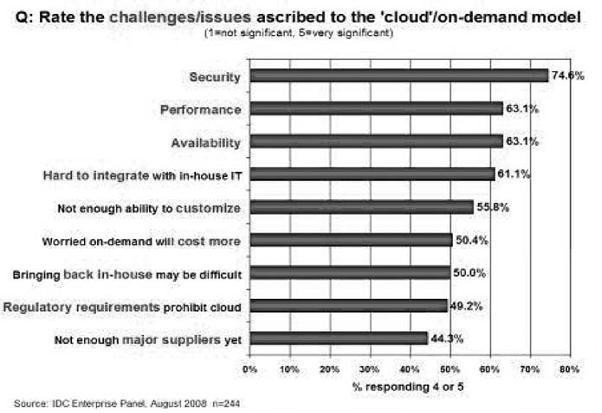
\includegraphics[scale=1]{gambar28.jpg} \\
\textbf{Gambar  2.8} Hasil survey tantangan keamanan IDC(\textit{International Data Corporation})
\end{center}

Terinspirasi oleh pergerakan industri \textit{IT} menuju SaaS, di mana perangkat lunak  tidak  dibeli, tetapi menyewa layanan dari penyedia, \textit{IT-as-a-Service} (ITaaS) sedang diusulkan untuk mengambil konsep ini lebih lanjut, untuk membawa hak model layanan untuk Infrastruktur TI anda. organisasi \textit{IT} modern harus menjalankan dirinya sebagai operasi yang terpisah dan menjadi  lebih strategis dalam pengambilan keputusan operasional.\\
Banyak organisasi dalam proses transformasi departemen IT mereka ke pusat biaya  operasional mandiri, memperlakukan pengguna internal yang seolah-olah mereka adalah pelanggan.\\
\tab Transformasi ini tidak sepele dan biasanya melibatkan unsur-unsur manajemen proyek portofolio, alur kerja rekayasa ulang, dan perbaikan proses. Transformasi ini memerlukan waktu yang lama untuk diselesaikan. Banyak organisasi IT besar yang telah mengadopsi  kerangka kerja \textit{Information Technology Infrastructure Library} (ITIL) dengan maksud membantu melalui trasformasi ini.\\\\
\textbf{Tantangan Keamanan \textit{Cloud}}\\\\
Meskipun virtualisasi dan komputasi awan dapat membantu perusahaan mencapai /melakukan sesuatu yang lebih dengan melanggar ikatan fisik antara infrastruktur \textit{IT} dan penggunanya, ancaman keamanan yang tinggi harus diatasi dalam rangka untuk mendapatkan manfaat sepenuhnya dari paradigma komputasi baru. Hal ini terutama berlaku untuk penyedia SaaS. Beberapa kekhawatiran keamanan adalah diskusi bernilai lebih. Sebagai contoh, di awan, Anda kehilangan kendali atas aset dalam beberapa hal, sehingga model keamanan Anda harus ditinjau kembali. Keamanan yang baik bagi perusahaan adalah yang menjadi mitra, department yang dapat diandalkan atau dipercaya. Dapatkah Anda mempercayai data Anda ke penyedia layanan Anda? Dalam paragraf berikut, kita membahas beberapa isu yang harus Anda pertimbangkan sebelummenjawab  pertanyaan.\\
\tab Dengan model awan, Anda kehilangan kontrol atas keamanan fisik. Dalam awan umum, Anda berbagi sumber daya komputasi dengan perusahaan lain. Di luar perusahaan anda tidak memiliki pengetahuan atau kendali dimana sumber daya dijalankan. Mengekspos data anda dalam lingkungan bersama dengan perusahaan lain , menjadikan "alasan yang masuk  akal" bagi pemerintah untuk menyita aset Anda karena perusahaan lain tersebut telah melanggar hukum. Hanya karena Anda berbagi lingkungan/tempat/ruangan di awan, dapat menempatkan data Anda pada resiko penyitaan/penyerangan.\\
\tab Layanan Penyimpanan yang disediakan oleh satu vendor awan mungkin tidak kompatibel dengan layanan vendor lain namun disatu sisi anda harus memutuskan untuk berpindah dari satu ke yang lain, dalamrangka memenuhi kebutuhan perusahaan anda.\\
Jika informasi dienkripsi saat melewati awan(\textit{Cloud}), siap yang mengontrol kunci enkripsi / dekripsi? Apakah pelanggan atau perusahaan \textit{Cloud} ? kebanyakan nasabah  mungkin  ingin data mereka dienkripsi dengan dua tipe control diatas (pengontrolan oleh pelanggan atau perusahaan \textit{Cloud}) di internet menggunakan SSL (\textit{Secure Sockets  Layer  protocol}).  Mereka juga mungkin ingin data mereka terenkripsi ketika sedang beristirahat di pool penyimpanan perusahaan awan(\textit{Cloud}). Pastikan anda sebagai pelanggan mengontrol kunci enkripsi/dekripsi, sama seperti ketika data masih tinggal di server anda sendiri.\\
\tab Integritas data artinya: memastikan bahwa data yang identik dijaga selama operasi apapun (seperti transfer, penyimpanan, atau pengambilan). Secara sederhana, integritas data adalah jaminan bahwa data konsisten dan benar. Memastikan keutuhan benar-benar dari data berarti bahwa perubahan hanya sebagai respons terhadap transaksi yang berwenang. Ini kedengarannya bagus, tetapi Anda harus ingat bahwa standar umum untuk  memastikan integritas data belum ada. Menggunakan penawaran SaaS di awan berarti bahwa ada sedikit kebutuhan untuk pengembangan perangkat lunak. Jika Anda berencana untuk menggunakan kode yang dikembangkan secara internal di awan(\textit{Cloud}), bahkan lebih penting untuk memiliki siklus pengembangan  perangkat  lunak  yang  aman  secara formal.  Penggunaan "teknologi mashup" yang belum matang (kombinasi layanan web), yang merupakan dasar aplikasi awan (\textit{Cloud}),tanpa disadari akan menyebabkan kerentanan keamanan dalam aplikasi tersebut. Pengembangan alat pilihan Anda , harus memiliki model keamanan yang tertanam/ melekat di dalamnya untuk membimbing pengembang dalam tahap pengembangan dan membatasi user dalampenggunaan data resmi mereka ketika sistemsedang digunakan di dalamproduksi.\\
\tab Aplikasi Awan(\textit{Cloud}) mengalami penambahan fitur yang konstan, dan pengguna harus terus up to date dengan perbaikan aplikasi untuk memastikan bahwa mereka dilindungi. kecepatan aplikasi yang akan berubah dalam awan(\textit{Cloud}) akan  mempengaruhi  SDLC (software    development     life    cycle)dan  keamanan. Sebagai     contoh,     Microsoft SDLC mengasumsikan bahwa misi penting perangkat lunak akan memiliki tiga sampai lima tahun periode dimana ia tidak akan berubah secara substansial, namun Awan (\textit{Cloud}) mungkin memerlukan perubahan aplikasi setiap beberapa minggu sekali. lebih buruk lagi, SLDC yang aman tidak akan mampu memberi siklus keamanan yang terus menerus terjaga dengan perubahan yang terjadi begitu cepat. Ini berarti bahwa pengguna harus terus-menerus upgrade, karena versi lama tidak dapat berfungsi, atau tidak dapat melindungi  data.\\
\tab Disini akan diambil contoh keamanan pada Layanan SaaS (\textit{Software as a Service}). Model \textit{Cloud computing} masa depan kemungkinan besar akan menggabungkan penggunaan SaaS, utilitas komputasi, dan kolaborasi teknologi Web 2.0 untuk memanfaatkan Internet untuk memenuhi  kebutuhan pelanggan mereka.\\
Model bisnis baru yang dikembangkan sebagai hasil dari peralihan ke \textit{Cloud Computing} tidak hanya menciptakan teknologi baru dan proses operasional bisnis tetapi juga persyaratan keamanan baru dan tantangan yang baru. Sebagai langkah evolusi terbaru dalam model layan \textit{Cloud} (seperti gambar di bawah ini), SaaS kemungkinan akan tetap menjadi model layanan awan yang dominan untuk masa yang akan datang dan sebagai tempat kebutuhan yang paling penting untuk praktik keamanan dan pengawasan.\\
\begin{center}
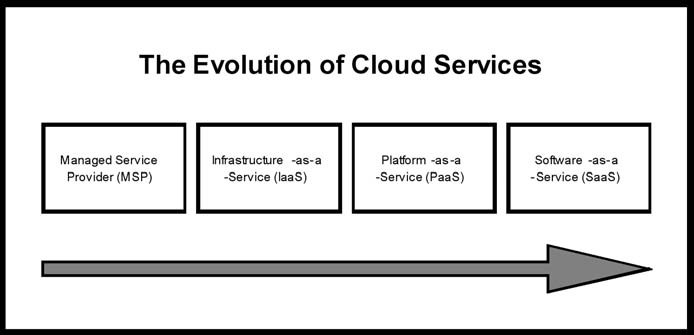
\includegraphics[scale=1]{gambar29.jpg} \\
\textbf{Gambar  2.9} Evolusi Layanan Awan. 
\end{center}
Seperti halnya dengan penyedia layanan yang diatur, perusahaan atau pengguna akhir perlu kebijakan penelitian vendor pada keamanan data sebelum menggunakan jasa vendor untuk menghindari  kehilangan atau tidak dapat mengakses data mereka.\\
Analis teknologi dan perusahaan konsultan Gartner mendaftar tujuh isu keamanan yang mana salah satu diantaranya  harus dibahas dengan perusahaan \textit{Cloud Computing} :\\
\begin{enumerate}
\item \textbf{Hak istimewa dari pengguna akses.}\\
Menanyakan tentang siapa yang memiliki akses khusus untuk data, dan tentang pengangkatan dan pengelolaan administrator tersebut.
\item \textbf{Peraturan kepatuhan.}\\
Pastikan bahwa vendor bersedia untuk menjalani audit eksternal dan / atau sertifikasi keamanan.
\item \textbf{Lokasi data.}\\
Apakah   penyedia   layanan   dalam   hal   ini   perusahaan   \textit{Cloud  Computing} melakukan pengendalian terhadap lokasi data.
\item \textbf{Pembagian / pemisahan data.}\\
Pastikan bahwa enkripsi tersedia di semua tahapan, dan bahwa skema enkripsi dirancang dan diuji  oleh para profesional berpengalaman.
\item \textbf{Pemulihanan / pembaruan.}\\
Cari tahu apa yang akan terjadi pada data sewaktu terjadi bencana / kerusakan. Mereka menawarkan pemulihan lengkap? Jika demikian, berapa lama waktu yang dibutuhkan untuk pemulihan tersebut sehingga pengguna layanan dapat menerima / mengambil data mereka sesuai kebutuhan denganmcepat dan tepat.
\item \textbf{Bantuan investigasi / bantuan penyelidikan.}\\
Apakah vendor memiliki kemampuan untuk menyelidiki setiap kegiatan  yang  tidak  patut atau ilegal?
\item \textbf{Kelayakan / kelangsungan jangka panjang.}\\
Apa yang akan terjadi pada data jika perusahaan yang bersangkutan(vendor) keluar/berhenti  dari bisnis? Bagaimana data yang dikembalikan, dan dalamformat apa?
\end{enumerate}
Menentukan jaminan keamanan data untuk jaman sekarang(hari-hari ini) begitu sulit, sehingga fungsi keamanan data menjadi begitu penting dibandingkan masa lalu. Taktik yang tidak terhandle oleh Gartner adalah meng-enkripsi data diri anda. Jika Anda mengenkripsi data menggunakan algoritma yang terpercaya, maka terlepas dari keamanan penyedia layanan dan kebijakan enkripsi, data hanya akan dapat diakses dengan kunci dekripsi.Tentu saja, ini mengarah ke tindak lanjut pada masalah: Bagaimana Anda mengelola kunci pribadi dalam infrastruktur komputasi  \textit{pay-on-demand} ?\\\\
\textbf{Masalah  keamanan data \textit{Cloud Computing.}}
\begin{enumerate}[label=\alph*]
\item \textbf{Masalah keamanan dari Virtual  machine.}\\\\
Apakah \textit{Blue Cloud} IBMatau Windows Azure di Microsoft, teknologi mesin virtual dianggap sebagai platform komputasi awan dari komponen fundamental, perbedaan antara \textit{Blue Cloud} dan Windows Azure adalah bahwa virtual mesin berjalan pada sistem operasi Linux atau sistem operasi Microsoft Windows. Teknologi virtual mesin membawa keuntungan yang nyata, ini memungkinkan pengoperasian server tidak lagi bergantung pada perangkat fisik. Tapi pada server virtual.  Pada  mesin virtual, perubahan yang fisik terjadi atau migrasi tidak  mempengaruhi layanan yang diberikan oleh penyedia layanan. jika pengguna membutuhkan jasa lebih, penyedia dapat memenuhi kebutuhan pengguna tanpa harus memperhatikan perangkat keras fisik.\\
\tab Namun, server virtual dari kelompok server logis membawa banyak masalah keamanan. Pengamanan terhadap pusat data tradisional diukur pada platformperangkat keras, sementara \textit{Cloud Computing} mungkin merupakan server dari   beberapa server virtual, server virtual mungkin milik kelompok server yang berbeda logis, server virtual, sehingga ada kemungkinan saling menyerang, yang membawa server virtual pada banyak ancaman keamanan.\\
Virtual mesin membentang pada tepi \textit{Cloud} yang membuat hilangnya batas jaringan sehingga mempengaruhi hampir semua aspek keamanan, isolasi fisik tradisional dan infrastruktur keamanan berbasis hardware tidak dapat menghentikan lingkungan komputer \textit{Cloud} yang saling menyerang antara virtual mesin.\\
\item \textbf{Keberadaan super – user.}\\\\
Untuk perusahaan yang menyediakan layanan komputasi awan (\textit{Cloud Computing}), mereka memiliki hak untuk melaksanakan pengelolaan dan pemeliharaan data, adanya super-user sangat bermanfaat untuk menyederhanakan fungsi manajemen data, tetapi merupakan  ancaman serius bagi pengguna pribadi. Dalam era privasi pribadi, data pribadi harus benar- benar dilindungi, dan fakta membuktikan bahwa \textit{platform  Cloud  Computing} memberikan layanan pribadi dalam kerahasiannya. Bukan hanya pengguna individu tetapi juga organisasi memiliki potensi ancaman serupa, misalnya pengguna korporat dan rahasia dagang disimpan dalam platform komputasi awan mungkin dicuri. Oleh karena itu penggunaan hak super user harus dikendalikan di awan(\textit{Cloud}).
\item \textbf{Konsistensi data.}\\\\
Lingkungan Awan (\textit{Cloud}) merupakan lingkungan yang dinamis, dimana data pengguna mentransmisikan data dari data center ke pengguna. Untuk sistem, data pengguna berubah sepanjang waktu. Membaca dan menulis data berkaitan dengan identitas otentikasi pengguna dan hal perijinan. Dalamsebuah mesin virtual, mungkin ada data pengguna yang berbeda 'yang harus wajib dikelola. Model  kontrol akses tradisional  dibangun di  "tepi" komputer, sehingga sangat lemah untuk mengendalikan pembaca dan penulis di antar komputer   yang terdistribusi.\\
\tab Hal ini jelas bahwa kontrol akses tradisional, jelas sangat tidak cocok untuk lingkungan komputasi awan. Dalam lingkungan komputasi awan, mekanisme kontrol akses tradisional memiliki  kekurangan serius.\\
\end{enumerate}
Prinsip keamanan data.\\\\
Semua teknik keamanan data dibangun pada kerahasiaan, integritas dan ketersediaan dari tiga prinsip dasar. Kerahasiaan mengacu pada apa yang disebut dengan data aktual atau informasi yang tersembunyi, terutama pada daerah yang sensitive, kerahasian data berada pada persyaratan yang lebih ketat. Untuk komputasi awan, data disimpan di "pusat data", keamanan dan kerahasiaan data pengguna, merupakan hal  yang penting.\\\\
Model  keamanan data.\\\\
Berikut gambar  model  keamanan data pada \textit{Cloud Computing}.\\
\begin{center}
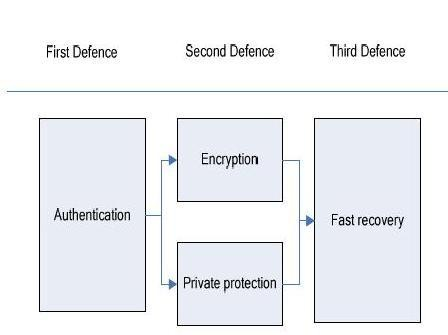
\includegraphics[scale=1]{gambar210.jpg} \\
\textbf{Gambar  2.10} Model Keamanan Data. 
\end{center}
Model struktur yang digunakan adalah system pertahanan tiga tingkat. di mana setiap tingkat melakukan tugas masing-masing untuk memastikan keamanan data dari lapisan awan(\textit{cloud}). Lapisan pertama: bertanggung jawab untuk otentikasi pengguna, pengguna  sertifikat  digital  yang diterbitkan oleh yang sesuai/berwenang, mengatur  hak akses pengguna.\\
Lapisan kedua: bertanggung jawab untuk enkripsi data pengguna, dan melindungi privasi dari pengguna melalui cara tertentu;\\
Lapisan ketiga: Data pengguna untuk pemulihan sistem yang cepat, perlindungan sistem lapisan terakhir dari data pengguna.\\\\
Kesimpulan :\\\\
Sebagai pengembangan komputasi awan, masalah keamanan telah menjadi prioritas utama. Akhirnya kami menyimpulkan teknologi komputasi awan ini sangat tepat untuk  menjaga keamanan data.